\documentclass[a4paper,11pt,twoside]{article}
\usepackage[T1]{fontenc}
\usepackage{subcaption}
\usepackage[utf8]{inputenc}
\usepackage{ngerman, eucal, mathrsfs, amsfonts, bbm, amsmath, amssymb, stmaryrd,graphicx, array, geometry, color, wrapfig, float, hyperref}
\geometry{left=25mm, right=15mm, bottom=25mm}
\setlength{\parindent}{0em} 
\setlength{\headheight}{0em} 
\title{Machine Learning\\ Blatt 4}
\author{Markus Vieth, David Klopp, Christian Stricker}
\date{\today}
\usepackage{listings, textcomp}
\usepackage[usenames,dvipsnames,svgnames,table]{xcolor}


\definecolor{Code}{rgb}{0,0,0}
\definecolor{Keywords}{rgb}{0,0,255}
\definecolor{Strings}{rgb}{255,0,0}
\colorlet{Comments}{Green}
\colorlet{Numbers}{blue}

%%%%%%%%%%%
%Mache Integer farbig
%%%%%%%%%%%

\makeatletter

\newif\iffirstchar\firstchartrue
\newif\ifstartedbyadigit

\newcommand\processletter
{%
	\ifnum\lst@mode=\lst@Pmode%
	\iffirstchar%
	\global\startedbyadigitfalse%
	\fi
	\global\firstcharfalse%
	\fi
}

\newcommand\processdigit
{%
	\ifnum\lst@mode=\lst@Pmode%
	\iffirstchar%
	\global\startedbyadigittrue%
	\fi
	\global\firstcharfalse%
	\fi
}

\lst@AddToHook{Output}%
{%
	\ifstartedbyadigit%
	\def\lst@thestyle{\color{Numbers}}%
	\fi
	\global\firstchartrue%
	\global\startedbyadigitfalse%
}

\newtoks\jubo@toks
\jubo@toks={
	language=C,
	commentstyle=\color{Comments}\slshape,
	stringstyle=\color{Strings},
	keywordstyle={\color{Keywords}\bfseries},
	alsoletter=0123456789,
	SelectCharTable=%
}
\def\add@savedef#1#2{%
	\begingroup\lccode`?=#1\relax
	\lowercase{\endgroup
		\edef\@temp{%
			\noexpand\lst@DefSaveDef{\number#1}%
			\expandafter\noexpand\csname lsts@?\endcsname{%
				\expandafter\noexpand\csname lsts@?\endcsname\noexpand#2}%
		}}%
		\jubo@toks=\expandafter{\the\expandafter\jubo@toks\@temp}%
	}
	\count@=`0
	\loop
	\add@savedef\count@\processdigit
	\ifnum\count@<`9
	\advance\count@\@ne
	\repeat
	\count@=`A
	\loop
	\add@savedef\count@\processletter
	\ifnum\count@<`Z
	\advance\count@\@ne
	\repeat
	\count@=`a
	\loop
	\add@savedef\count@\processletter
	\ifnum\count@<`z
	\advance\count@\@ne
	\repeat
	%\showthe\jubo@toks % for debugging
	\begingroup\edef\x{\endgroup
		\noexpand\lstdefinestyle{pseudo}{\the\jubo@toks}
	}\x
	
	\makeatother
%%%%%%%%%%
%Ende
%%%%%%%%%%



\lstset{
	literate={ö}{{\"o}}1
	{ä}{{\"a}}1
	{ü}{{\"u}}1
	{ß}{{\ss}}1
	{/pi}{{$\Pi$}}1
	{/inf}{{$\infty$}}1
	{/eIn}{{$\in$}}1
	{/cup}{{$\cup$}}1
	{/leer}{{$\emptyset$}}1
	{<=}{{$\leq$}}1
	{>=}{{$\geq$}}1
}


\lstset{
	numberstyle=\tiny,
	stepnumber=1,
	numbersep=10pt,
	xleftmargin=15pt,
	breaklines=true,
	numberblanklines=false,
	showstringspaces=false,
	flexiblecolumns=true,
	mathescape=true,
	tabsize=4,
	captionpos=b,
	numbers=left,
	commentstyle=\color{Green},
	numberstyle=\color{gray},
	keywordstyle=\color{blue} \textbf,%otherkeywords={xdata},
	keywords=[2]{xdata},
	keywordstyle=[2]\color{red}\textbf,
	identifierstyle=\color{black},
	stringstyle=\color{red}\ttfamily,
	basicstyle = \ttfamily \color{black} \footnotesize,
	inputencoding=utf8,
	emph=[1]%
	{%
		infinity,
	}, 
	emphstyle=[1]{\color{blue}},
	emph=[2]%
	{%
		forall,
		while,
		if,
		else,
		for,
		return,
		new,
		NULL,
		null,
		int, 
		double, 
		float,
		class,
		void,
		false, 
		true,
		FALSE,
		TRUE,
	}, 
	emphstyle=[2]{\color{Magenta}},
	emph=[3]{b0, b1, n0, n1},
	emphstyle=[3]{\color{black}}
}
\begin{document}

\newcommand{\cor}[1]{\textcolor{red}{\textit{#1}}}
\maketitle
\cleardoublepage
\pagestyle{myheadings}
\markboth{Markus Vieth,  David Klopp, Christian Stricker}{Markus Vieth, David Klopp, Christian Stricker}

\newpage

\section*{Nr.1}
\begin{figure*}[h]
	\captionsetup[subfigure]{labelformat=empty}
	\centering
	\begin{subfigure}[t]{0.33\textwidth}
		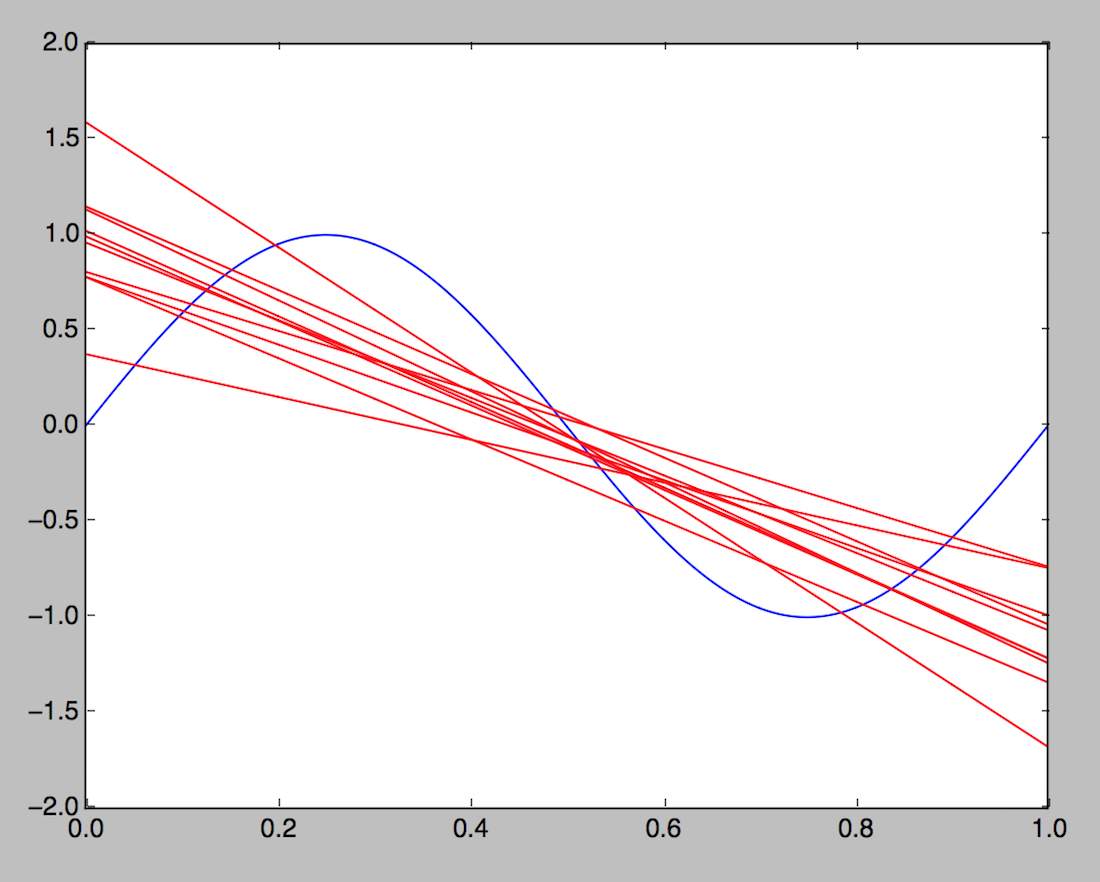
\includegraphics[width=\textwidth]{images/Nr_1/d_1.png}
		\caption{Abbildung 1: d=1}
	\end{subfigure}%
	~
	\begin{subfigure}[t]{0.33\textwidth}
		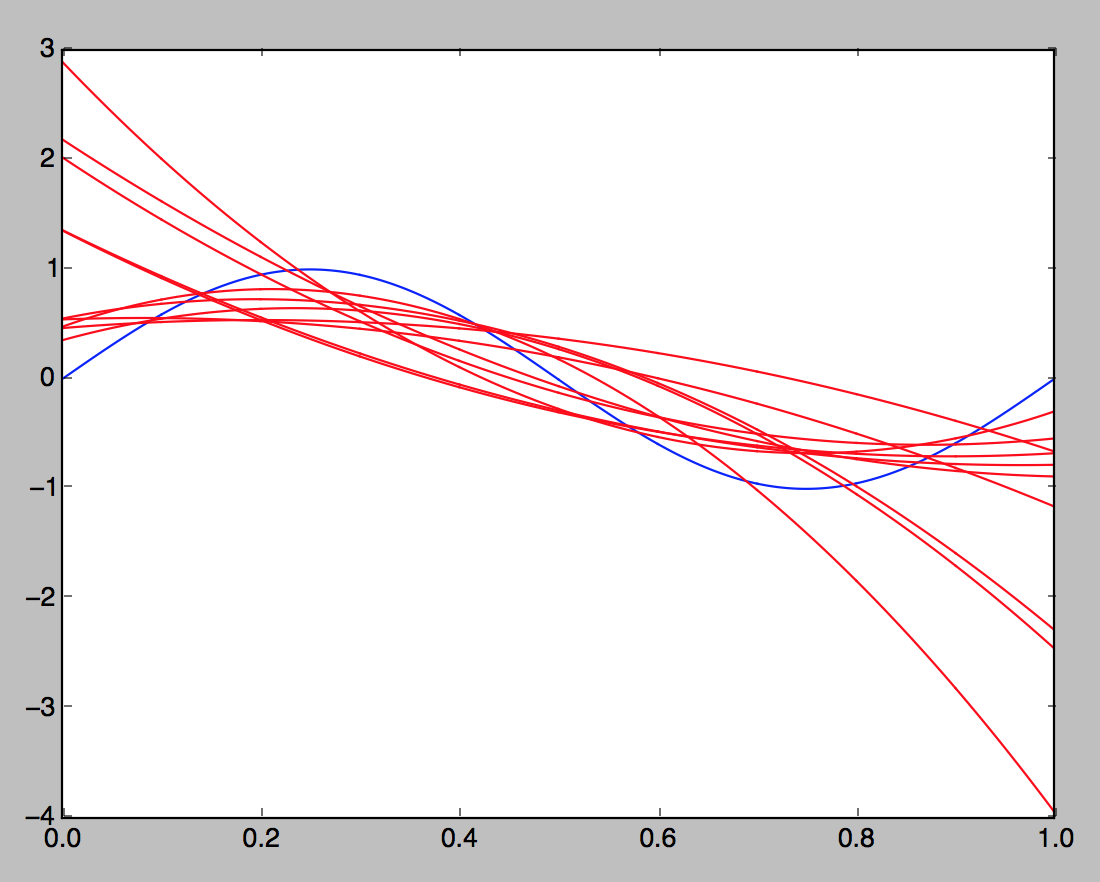
\includegraphics[width=\textwidth]{images/Nr_1/d_2.png}
		\caption{Abbildung 2: d=2}
	\end{subfigure}%
	~
	\begin{subfigure}[t]{0.33\textwidth}
		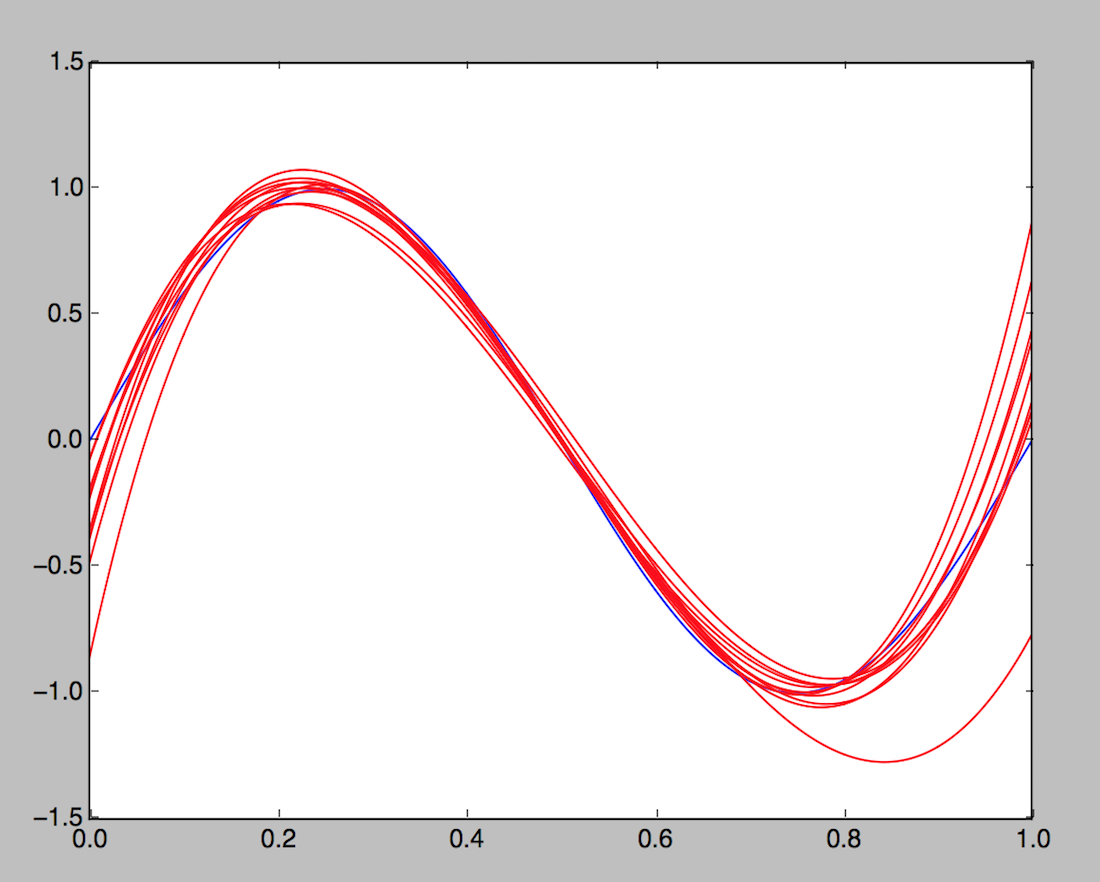
\includegraphics[width=\textwidth]{images/Nr_1/d_3.png}
		\caption{Abbildung 3: d=3}
	\end{subfigure}
\end{figure*}

\begin{figure*}[h]
	\captionsetup[subfigure]{labelformat=empty}
	\centering
	\begin{subfigure}[t]{0.33\textwidth}
		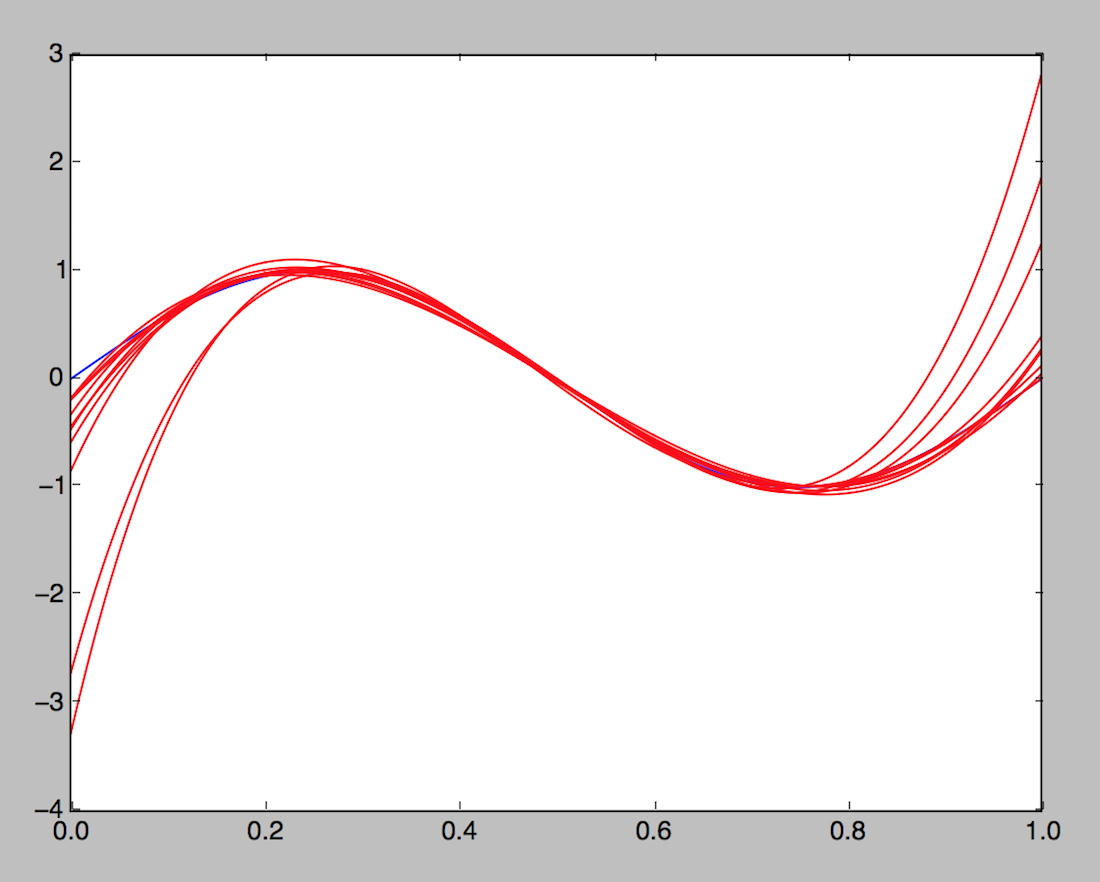
\includegraphics[width=\textwidth]{images/Nr_1/d_4.png}
		\caption{Abbildung 4: d=4}
	\end{subfigure}%
	~
	\begin{subfigure}[t]{0.33\textwidth}
		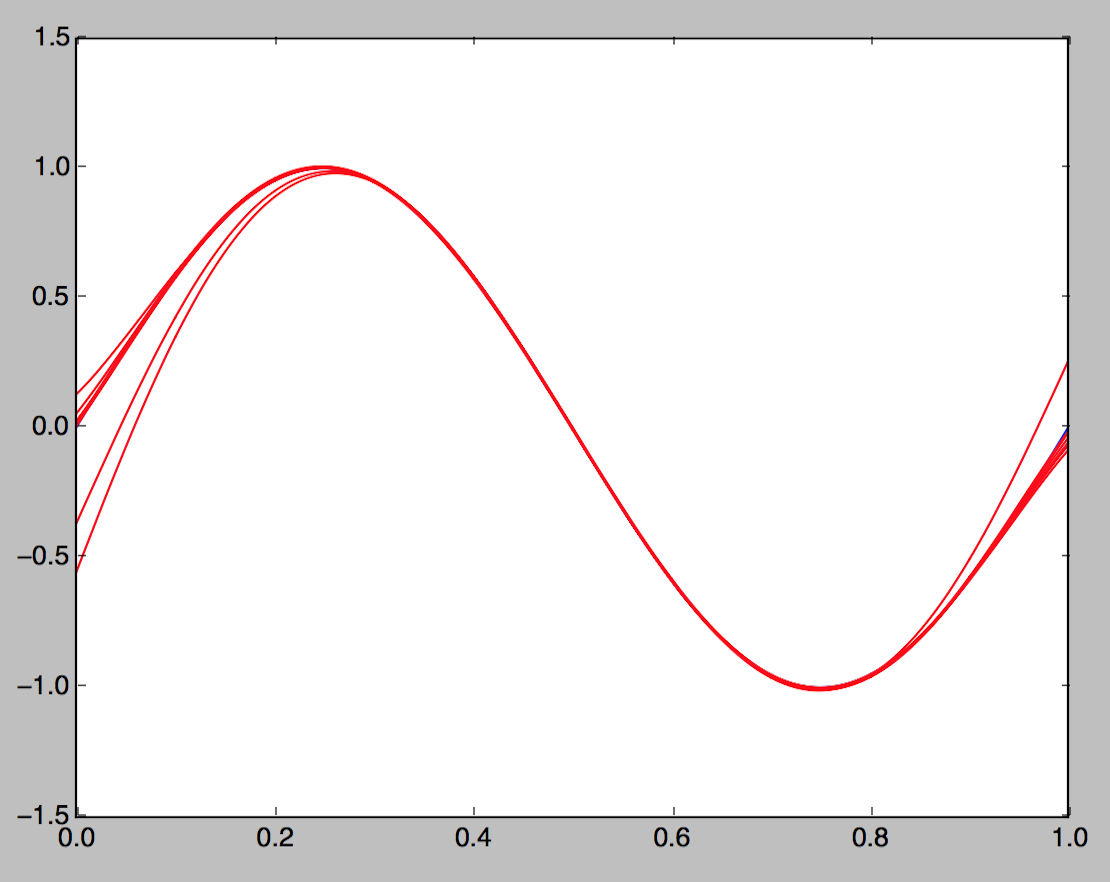
\includegraphics[width=\textwidth]{images/Nr_1/d_5.png}
		\caption{Abbildung 5: d=5}
	\end{subfigure}%
	~
	\begin{subfigure}[t]{0.33\textwidth}
		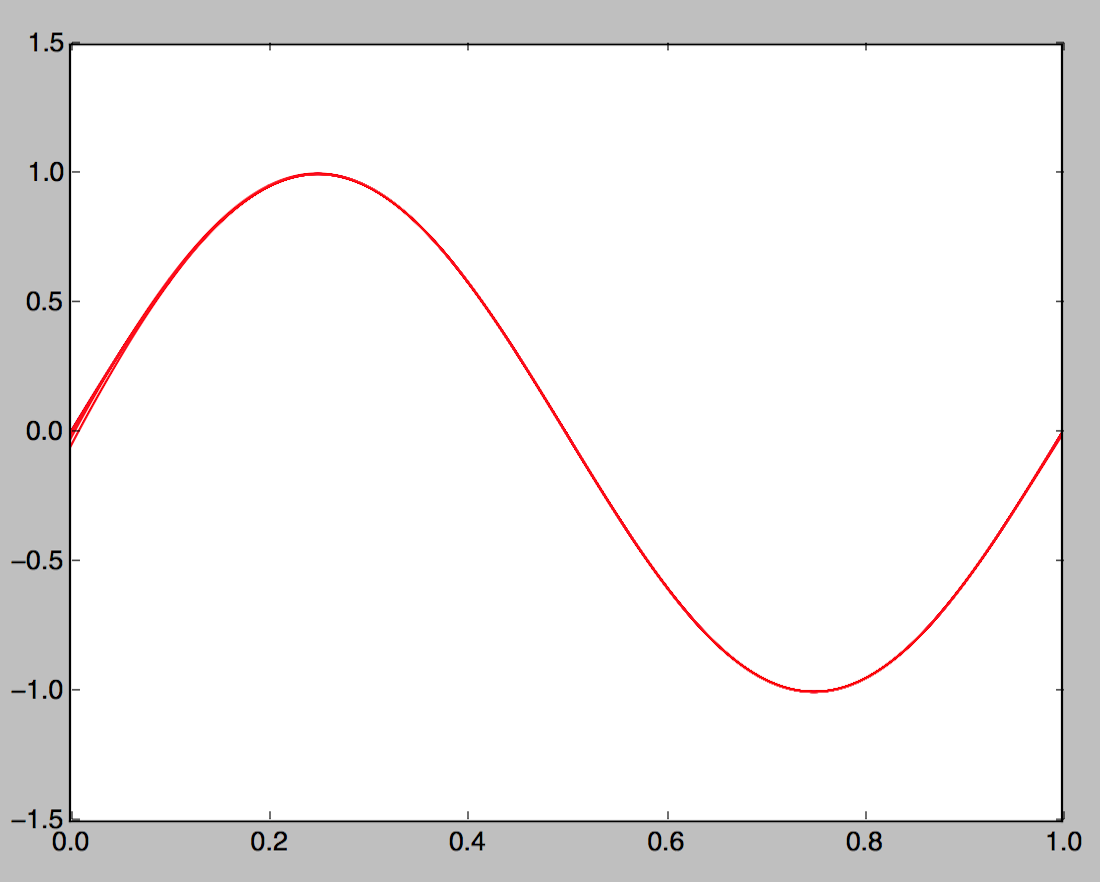
\includegraphics[width=\textwidth]{images/Nr_1/d_10.png}
		\caption{Abbildung 6: d=10}
	\end{subfigure}
\end{figure*}

Die Grafiken verdeutlichen, dass der Bias zu Beginn sehr hoch ist, da der Sinus nicht durch eine Funktion ersten Gerades akkurat angenähert werden kann. Je höher man nun den Wert d, also den Grad des Polynoms zum annähern wählt, desto präziser kann die Sinus-Funktion approximiert werden und desto kleiner wird der Bias. Die Varianz lässt sich in den angegebenen Abbildungen nur schwer erkennen. In Abbildung 6 im Interval 0 bis 0.2, lässt sich eine leichte Streuung erkennen, die durch das Rauschen der Trainingsdaten verursacht worden sein könnte. Diese leichte Streuung kann allerdings auch durch den immer noch zu geringen Grad d des Polynoms entstanden sein.


\section*{Nr.2}
\begin{figure}[H]
	\centering
	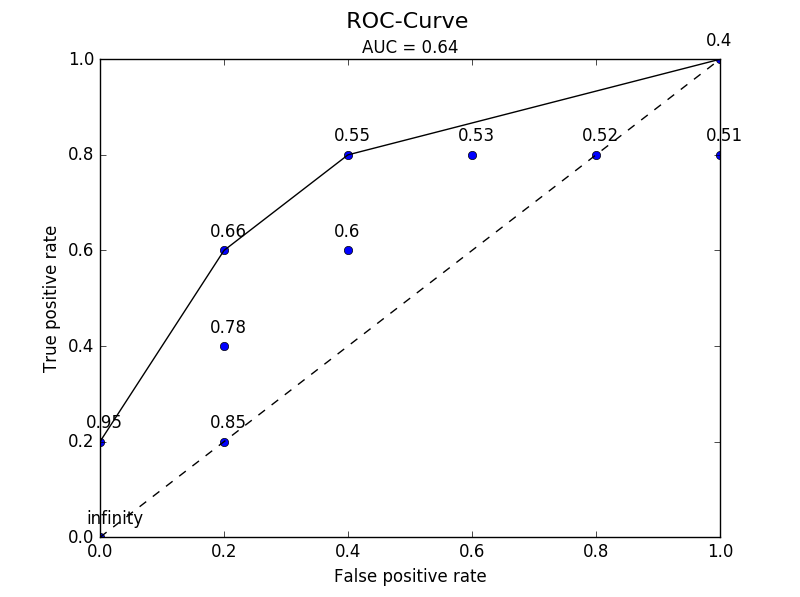
\includegraphics[width=\textwidth]{images/figure_1.png}
	\caption{ROC-Curve with convex hull}
\end{figure}
Anhand des Graphen ist zu sehen, dass der Classifier besser ist, als einfaches, gleichverteiltes raten (gestrichelte Linie). Ebenfalls geht hervor, dass der Classifier eher richtig als falsch klassifiziert, da die Kurve fast konkav ist. Eine AUC von wie hier $0,64$ ist nicht besonders gut, da dies bedeutet, dass das die Wahrscheinlichkeit für ein zufälliges positives Beispiel aus dem Datensatz einen kleineren Score zu haben als für ein zufälliges negatives Beispiel bei über $35\%$ liegt. Hier wäre ein höherer Wert wünschenswert. Im Allgemeinen handelt es sich hier um einen schlechten Classifier (vergleiche \url{http://mlwiki.org/index.php/ROC_Analysis}).  
\pagebreak
\section*{Nr.3}
\lstinputlisting[language = java]{code/Nr3.java}


\section*{Nr.4}
Quellcode zu den Aufgaben aufgrund des Umfangs digital.
\subsection*{a)}
Es wurden folgende Datensätze gewählt:
\begin{itemize}
	\item splice.arff
	\item letter.arff
	\item kr-vs-kp.arff
\end{itemize}
\pagebreak
\subsection*{b)}
Die Vergleiche brachten folgende Ergebnisse (Bootstrap.635-Validierung):\\
File res/letter.arff\\
0 = a = RandomForest\\
1 = b = J48 as DecisionTree\\
letzte McNema Tabelle\\
\begin{tabular}{rcc}
 &a falsch&a richtig\\
b falsch&244&64\\
b richtig&798&6288
\end{tabular}\\
avg. McNema Stat. over 10\\
$577.539575643173$\\
$~$\\
File res/kr-vs-kp.arff\\
0 = a = RandomForest\\
1 = b = J48 as DecisionTree\\
last McNema Table\\
\begin{tabular}{rcc}
	&a falsch&a richtig\\
	b falsch&2&6\\
	b richtig&3&1128
\end{tabular}\\
avg. McNema Stat. over 10\\
$2.1657428274340043$\\
$~$\\
File res/splice.arff\\
0 = a = RandomForest\\
1 = b = J48 as DecisionTree\\
last McNema Table\\
\begin{tabular}{rcc}
	&a falsch&a richtig\\
	b falsch&32&66\\
	b richtig&57&1016
\end{tabular}\\
avg. McNema Stat. over 10\\
$2.354155198842717$\\
\subsection*{c)}
Wie in den Vergleichen deutlich wird, lässt sich keine Allgemeine Aussage treffen. In 1 von 3 Fällen, war der RandomForest deutlich besser, während er in den anderen beiden Datensätzen sogar (unwesentlich) schlechter war als der DecisionTree.
\subsection*{d)}
Bei dem durchgeführten Experiment wurde klar, dass RandomForest nicht immer besser ist als ein DecisionTree. Die auffälligsten Unterschieden zwischen den Datensätzen 2 und 3 zu 1 ist, dass 1 im Vergleich viele Klassen besitzt. Auch die Anzahl der vorhandenen Instanzen ist um ein vielfaches Größer, was mich zu der Annahme verleitet, dass RandomForest auf einem begrenzten Datensatz seine Stärken zeigt, jedoch ein DecisionTree bei ausreichend vielen Trainingsdaten besser klassifizieren kann, weil dann zu ausreichend vielen Attributen eine Abhängigkeit erstellt werden kann (unter der Voraussetzung, dass die vorhandenen Attribute einen kausalen Zusammenhang zur Klasse haben).
\section*{Nr.5}
\[accuracy = \frac{TP + TN}{TP + FP + FN + TN}\]
\[= \frac{TP}{P+N} + \frac{TN}{P+N}\]
\[= \frac{P \cdot TP}{P \cdot (P+N)} + \frac{N \cdot TN}{N \cdot (P +N)}\]
\[= \frac{TP}{P} \cdot \frac{P}{P+N} + \frac{TN}{N} \cdot \frac{N}{P+N} \]
\[= \frac{TP}{P} \cdot \frac{P}{P+N} + \frac{TN}{N} \cdot \left(1- \frac{P}{P+N}\right) \]
Mit A = $\frac{P}{P+N}$ folgt: 
\[accuracy = sensitivity \cdot A + specificity \cdot (1-A)\]

\end{document}